\chapter{Firewalls, IDS and Web Security}
\section{Firewalls}
Un firewall è un componente passivo di difesa perimetrale di una rete informatica, che integra un insieme di misure progettate per prevenire l'accesso non autorizzato a tale rete. Letteralmente firewall significa \textit{muro tagliafuoco}, con riferimento ai muri refrattari costruiti nelle strutture per assicurarne l'isolamento.

\subsection{Firewall Policies}
Al fine di proteggere reti private o singole macchine dai pericoli di Internet, un firewall può essere utilizzato per filtrare il traffico in uscita o in entrata sulla base di un insieme di regole predefinite, denominate \textbf{firewall policies}.
I pacchetti che passano per un firewall possono essere:
\begin{itemize}
\item \textbf{Accepted}: il firewall ne permette il passaggio
\item \textbf{Dropped}: il passaggio non viene permesso e tale negazione non viene segnalata
\item  \textbf{Rejected}: il passaggio non viene permesso e il firewall tenta di informare la sorgente del rifiuto del pacchetto 
\end{itemize}
Le policies usate dal firewall per gestire il traffico sono basate su diverse proprietà dei pacchetti che vengono analizzati, incluso il protocollo usato, come:
\begin{itemize}
\item TCP o UDP
\item Gli indirizzi IP del mittente e del destinatario
\item Le porte di partenza e di destinazione del pacchetto
\item il payload del livello applicativo del pacchetto (ad esempio analizzando se contiene virus)
\end{itemize}
\subsubsection{Blacklist e Whitelist}
Vi sono due approcci fondamentali nella creazione delle policies che garantiscono la minimizzazione delle vulnerabilità esposte pur mantenendo le funzionalità desiderate:

\begin{itemize}
\item \textbf{Blacklist approach}: Tutti i pacchetti sono accettati, tranne quelli per cui sono verificate le condizioni specificate nella blacklist. Questo tipo di configurazione, \textbf{orientata al servizio}, è più flessibile nell'assicurare che le funzionalità desiderate non siano danneggiate dal firewall, ma dal punto di vista della sicurezza risulta un approccio "ingenuo": si assume che l'amministratore conosca tutte le possibili caratteristiche dell'eventuale traffico malevolo.

\item \textbf{Whitelist approach}: Un approccio più sicuro, \textbf{orientato alla sicurezza}, consiste nel rifiutare il traffico per default, in modo che i pacchetti siano rifiutati a meno che non rispondano a determinate condizioni specificate dal firewall. 
\end{itemize}

\subsection{Tipi di Firewall}
\begin{itemize}
\item \textbf{packet filters (stateless)}: Se un pacchetto soddisfa le regole definite dal packet filter, viene trattato di conseguenza (rifiutato o accettato a seconda dell'approccio utilizzato, i.e. blacklist o whitelist)
\item \textbf{"stateful" filters}: Questo tipo di firewall tiene traccia di tutte le connessioni che passano attraverso di esso, e può determinare se un pacchetto corrisponde all'apertura di una nuova connessione, se appartiene ad una connessione precedente o se è un pacchetto invalido.
\item \textbf{application layer}: Questo tipo di firewall funziona come un proxy, in modo da poter "capire" determinati protocolli o applicazioni. Può analizzare il contenuto del traffico, eventualmente bloccandolo in caso di contenuti sospetti (i.e. siti web, virus, vulnerabilità, ...).
\end{itemize}
\subsubsection{Stateless firewalls (Packet filters)}
Un firewall stateless non tiene in memoria nessuno stato rispetto ai pacchetti che processa. Tratta ogni pacchetto indipendentemente ed in maniera isolata dagli altri, senza considerare, ad esempio, se ha già processato lo stesso pacchetto in passato. \textbf{In genere i firewall stateless devono essere configurati in maniera abbastanza restrittiva affinché prevengano la maggior parte degli attacchi.}

\begin{figure}[htbp]
	\centering%
	\subfigure%
	{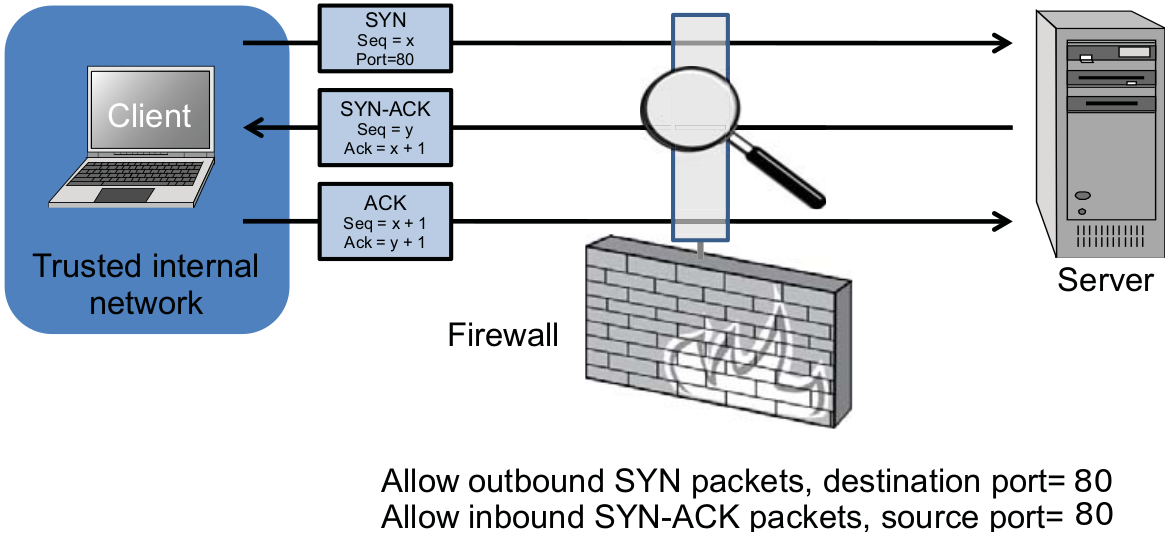
\includegraphics[height=13cm, width=13cm, keepaspectratio]{Immagini/firewalls/stateless_firewall.png}}
	\caption{Stateless firewall \label{fig:stateless_firewall}} 	
\end{figure}

\subsubsection{Stateful firewalls}
I firewall stateful sono in grado di riconoscere i pacchetti che fanno parte di una sessione legittima originata all'interno di una rete fidata. Essi tengono in memoria tabelle contenenti informazioni su ogni connessione attiva, come indirizzi IP, porte e numeri di sequenza dei pacchetti. Usando tali tabelle, questo tipo di firewall può permettere, ad esempio, solo il passaggio di pacchetti che rappresentano una risposta ad una connessione iniziata dall'interno della rete fidata.

\begin{figure}[htbp]
	\centering%
	\subfigure%
	{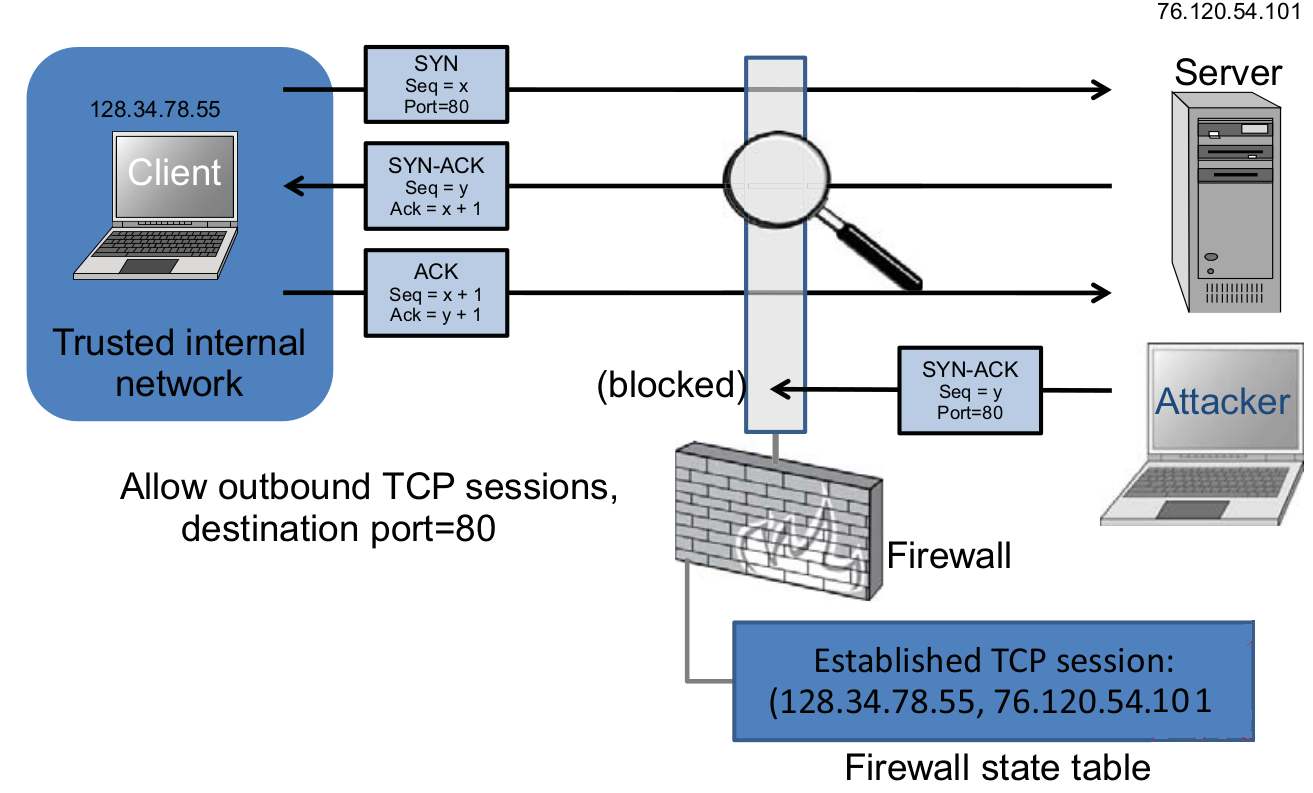
\includegraphics[height=13cm, width=13cm, keepaspectratio]{Immagini/firewalls/stateful_firewall.png}}
	\caption{Stateful firewall \label{fig:stateful_firewall}} 	
\end{figure}

\section{Tunnels}
Il contenuto dei normali pacchetti TCP non è solitamente crittografato. Se qualcuno pratica eavesdropping sulla connessione può spesso vedere il completo contenuto dei payloads della sessione. Un modo per prevenire questo tipo di attacco alla confidenzialità senza modifificare lo strato applicativo coinvolto nella sessione è utilizzare un \textbf{protocollo di tunneling}. In questo tipo di protocolli la comunicazione tra client e server è automaticamente crittografata, in modo da rendere infattibile l'eavesdropping.

\begin{figure}[htbp]
	\centering%
	\subfigure%
	{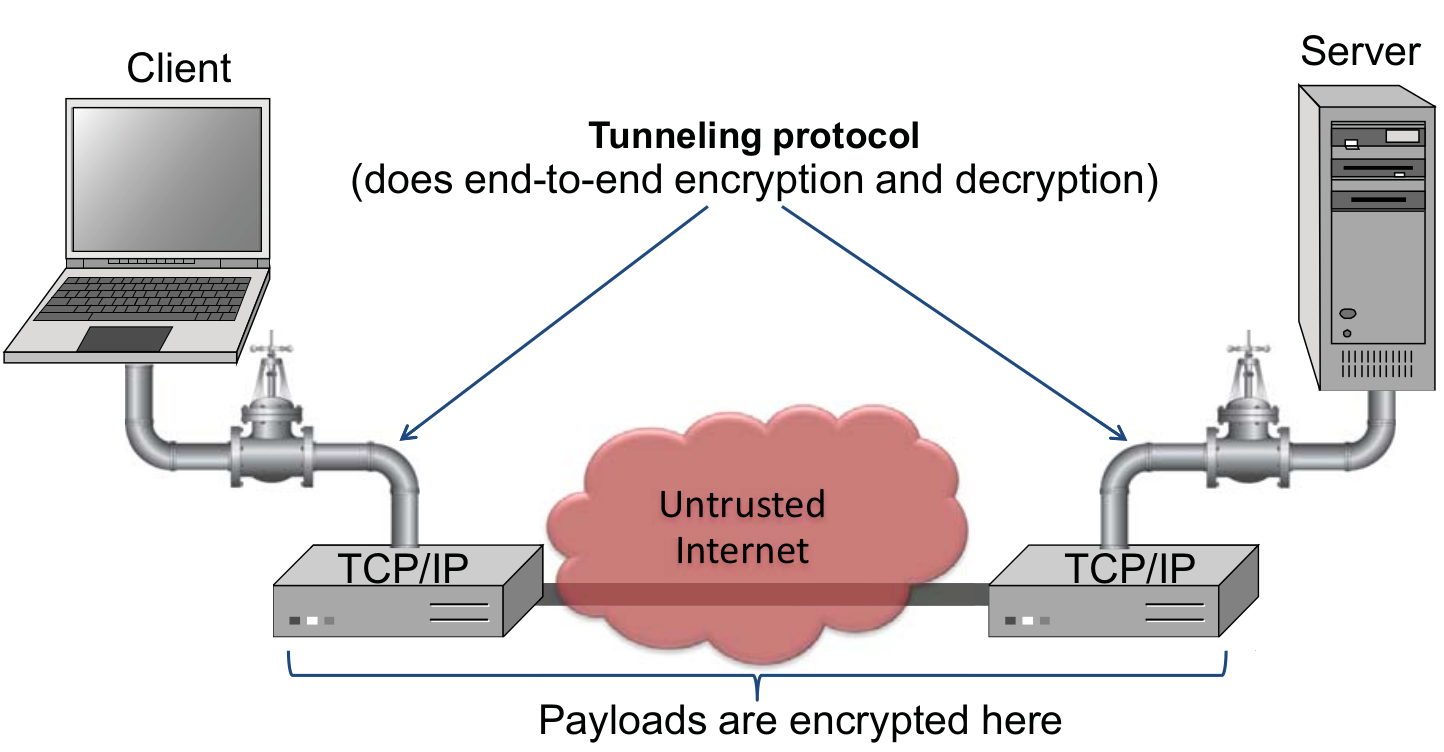
\includegraphics[height=13cm, width=13cm, keepaspectratio]{Immagini/firewalls/tunnel.png}}
	\caption{Stateful firewall \label{fig:tunnel}} 	
\end{figure}

\section{Intrusion Detection Systems (IDS)}
Un intrusion detection system (IDS) è un dispositivo o un'applicazione software che monitora le attività di un sistema o di una rete locale con l'obiettivo di identificare attività malevoli o violazione di policy, e produrre dei report a riguardo.
Alcune definizioni:
\begin{itemize}
\item \textbf{Intrusione}: Azione finalizzata alla compromissione della sicurezza dell'obiettivo (confidenzialità, integrità, disponibilità o risorse di rete e/o di calcolo)
\item \textbf{Intrusion detection}: L'identificazione, tramite segnali di intrusione e la relativa produzione di report a riguardo.
\item \textbf{Intrusion prevention}: Il processo che coinvolge sia la rivelazione di attività di intrusione sia la gestione automatica delle misure di reazione all'intrusione.
\end{itemize}

\subsection{Componenti di un IDS}
L'\textbf{IDS manager} processa i dati provenienti dai \textbf{sensori IDS} con il fine di determinare se è avvenuta un'intrusione. Tale rilevamento è basato su una serie di policy, ovvero di regole e condizioni che, se verificate, indicano una probabile intrusione. Una volta che il manager rileva un intrusione, scatta un allarme.

\begin{figure}[htbp]
	\centering
	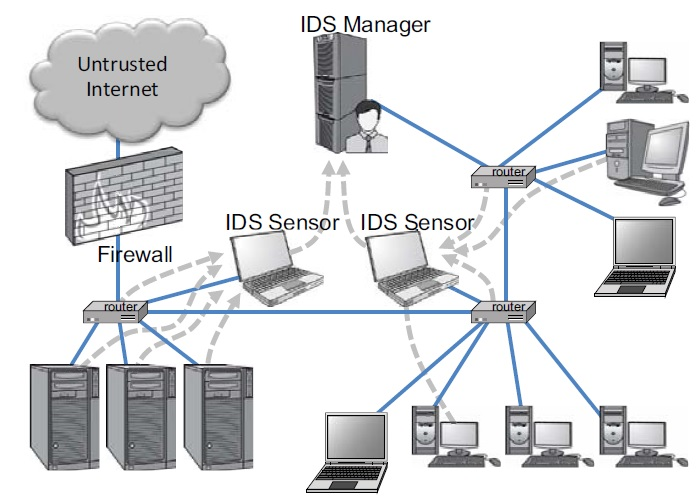
\includegraphics[width=0.5\linewidth]{Immagini/firewalls/IDS.png}
	\caption{IDS Components} 	
	\label{fig:IDS_components}
\end{figure}

\subsection{Intrusioni}
Un IDS è progettato al fine di rilevare una serie di minacce, tra cui le seguenti:

\begin{itemize}
\item \textbf{Masquerader}: un attaccante che sta utilizzando in maniera fraudolenta l'identità e/o le credenziali di un utente legittimo per ottenere accesso ad un computer o ad una rete
\item \textbf{Misfeasor}: un utente legittimo che sta eseguendo azioni che non è autorizzato ad eseguire
\item \textbf{Clandestine user}: un utente che prova a bloccare o mascherare le sue azioni eliminando file di audit e/o log di sistema
\end{itemize}

Inoltre un IDS può essere progettato al fine di rilevare i seguenti attacchi automatizzati:
\begin{itemize}
\item \textbf{Port scans}: raccolta di informazioni finalizzata a scoprire quali porte su una determinata interfaccia accettano connessioni TCP
\item \textbf{Denial-of-service attacks}: attacchi di rete finalizzati a saturare un host di richieste fino all'impossibilità di erogare il servizio che normalmente eroga
\item \textbf{Malware attacks}: Trojan horses, computer worms, virus, etc.
\item \textbf{ARP spoofing}: tentativi di reindirizzare traffico IP in una LAN
\item \textbf{DNS cache poisoning}: attacco che prevede la modifica della cache DNS di un host per creare una falsa associazione domain-name/IP-address 
\end{itemize}

\subsection{IDS Data} 
In una influente pubblicazione del 1987, Dorothy Denning identificò molti campi che dovrebbero essere inclusi nella registrazione degli eventi da parte di un IDS:
\begin{itemize}
\item \textbf{Subject}: l'iniziatore di un'azione sull'obiettivo
\item \textbf{Object}: la risorsa in questione, ad esempio un file, un comando, un device, o un protocollo di rete
\item \textbf{Action}: l'operazione eseguita dal subject verso l'object
\item \textbf{Exception-condition}: ogni messaggio di errore o eccezione sollevata dalla action
\item \textbf{Resource-usage}: misure quantitative delle risorse utilizzate dal sistema nell'effettuare la action
\item \textbf{Time-stamp}: un identificatore unico per l'istante in cui si inizia la action
\end{itemize}

\subsection{Tipi di Intrusion Detection Systems} 
\subsubsection{Rule-Based Intrusion Detection} 
Si definiscono delle regole che identificano i tipi di azioni che corrispondono ad un determinato profilo di attacco: una data regola codifica quindi una firma per uno specifico attacco. Se l'IDS manager rileva un evento che corrisponde alla firma per una data regola, farà suonare immediatamente un allarme, indicando possibilmente anche il tipo di attacco che si sospetta sia in atto.

\subsubsection{Statistical Intrusion Detection}
Viene creato un profilo che corrisponde alla rappresentazione statistica del modo un cui un utente interagisce con il sistema. Quando si imposta un dato profilo, l'IDS manager può determinare le soglie che definiscono i comportamenti anomali e quindi suonare un allarme ogni qual volta il comportamento di un utente devia in maniera significativa dallo standard definito dal profilo.

\section{Cross Site Scripting (XSS)}
Il Cross-site scripting è una vulnerabilità, tipicamente presente nelle applicazioni web, che permette ad hacker di iniettare uno script in una applicazione web vulnerabile, la quale inconsapevolmente farà eseguire lo script nel browser dei suoi utenti. XSS può essere usato per portare a compimento un insieme variegato di attacchi quali: phishing, hijacking, cambio delle impostazioni di utente, furto/avvelenamento di cookies, pubblicità ingannevole, esecuzione di codice lato client, etc. 
\begin{figure}[htbp]
	\centering
	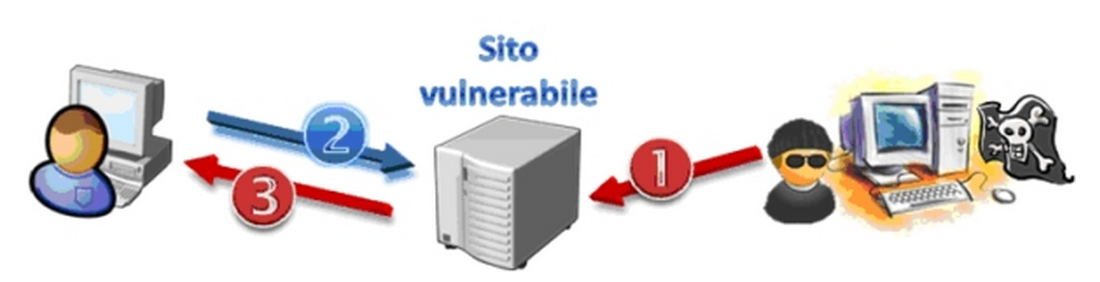
\includegraphics[width=0.5\linewidth]{Immagini/firewalls/XSS.png}
	\caption{Schema base di un attacco XSS} 	
	\label{fig:XSS_attack}
\end{figure}
\\
I metodi per iniettare codice malevolo sono di 3 tipi:
\begin{itemize}
	\item \textbf{DOM-based (“type 0”)}: 	L'attaccante memorizza il codice maligno a livello locale nel Document Object Model (DOM) utilizzato per la rappresentazione HTML o XML.
	\item \textbf{Reflected XSS (“type 1”)}: lo script attacco viene riflesso verso l'utente come parte di una pagina del sito vittima dell'attacco.
	\item \textbf{Stored XSS (“type 2”)}: l'attaccante memorizza il codice maligno in una risorsa gestita dall'applicazione web, ad esempio un database.
\end{itemize}
Possibili difese lato client sono le seguenti:
\begin{itemize}
	\item \textbf{Proxy-based}: analizzare il traffico HTTP scambiato tra il browser web dell'utente e il server web di destinazione mediante la ricerca di caratteri HTML speciali e conseguente codifica prima di eseguire la pagina sul browser dell'utente (ad esempio il plugin NoScript per Firefox).
	\item \textbf{Application-level firewall}: Analizzare le pagine HTML visitate mediante la ricerca di hyperlink che potrebbero portare a perdite di informazioni sensibili e stoppare le bad request utilizzando un insieme di regole di connessione.
	\item \textbf{Auditing system}: monitorare l'esecuzione di codice JavaScript e confrontare le operazioni con politiche di alto livello per rilevare comportamenti dannosi.
\end{itemize}

\section{SQL Injection Attack}
Molte applicazioni web ottengono gli input dell'utente da una form. Spesso questo input viene utilizzato, nella costruzione di una query SQL da sottoporre ad un database, in maniera letterale. Per esempio:
\begin{lstlisting}
SELECT user 
FROM table
WHERE name = 'user input name'
\end{lstlisting}
Un attacco di tipo SQL injection prevede l'inserimento di istruzioni SQL nell'input dell'utente.
\subsubsection{Login Query: username and password} 
Viene qui fornita una query standard per verificare se la correttezza della procedura di Login:
\begin{lstlisting}
SELECT * 
FROM users 
WHERE user = '$usern' AND pwd = '$password'
\end{lstlisting}
Se un attaccante inserisce i seguenti valori nei campi username/password:
\begin{lstlisting}
$usern = "M' OR '1=1"
$password = "M' OR '1 = 1"
\end{lstlisting}
Di conseguenza si ottiene:
\begin{lstlisting}
SELECT * 
FROM users 
WHERE user = 'M' OR '1=1' AND pwd = 'M' OR '1=1'
\end{lstlisting}
Risultato: ottiene l'accesso!\\
Un altra query:
\begin{lstlisting}
SELECT user, pwd 
FROM users 
WHERE user = '$usern' 
\end{lstlisting}
Se di nuovo:
\begin{lstlisting}
$usern = "M' OR '1=1" 
\end{lstlisting}
Risultato: si ottiene l'intera tabella!\\
Per evitare questo tipo di attacco è necessario controllare 2 cose: il risultato della query deve essere una singola tupla e inoltre tale risultato deve essere formalmente corretto. \\
\linebreak
Consideriamo un altro tipo di input malevolo, se fosse:  
\begin{lstlisting} 
$usern="M' ; drop table user;"
\end{lstlisting}
Si potrebbe utilizzare un \textbf{metodo di Escape} che sostituisce tutti i caratteri "malevoli".
Considerando ad esempio la seguente espressione:
\begin{lstlisting} 
Escape("t ' c") 
\end{lstlisting}
essa dà come risultato
\begin{lstlisting} 
"t \' c"
\end{lstlisting}
Quindi, scrivendo:
\begin{lstlisting} 
SELECT user, pwd 
FROM users 
WHERE user = '$usern'
\end{lstlisting}
e:
\begin{lstlisting} 
$usern = escape("M' ;drop table user;")
\end{lstlisting}
Dà come risulta la query sicura:
\begin{lstlisting} 
SELECT user, pwd 
FROM users 
WHERE user='M\'drop table user;\''
\end{lstlisting}
Possibili \textbf{soluzioni} per gli attacchi di tipo SQL injection sono: \textbf{Escape string} e \textbf{rigida verifica dei tipi}.